\documentclass{article}
\usepackage{bnaic}
\usepackage{graphicx}
\usepackage{mathtools}
\usepackage{amsmath}
\usepackage[table]{xcolor}
\usepackage{caption}

% ML Jun24: These comments are 
%\section{The bnaic Package}
%The \verb+bnaic.sty+ file is a package that is to be used together with
%the standard \verb+article+ document class. Please adhere strictly to the instructions of this document. The bnaic style file uses the standard \verb+times+ package and the \verb+geometry+ package, which is included in the bnaic package; please do not change it! 

%% if your are not using LaTeX2e use instead
%% \documentstyle[bnaic]{article}

%% begin document with title, author and affiliations


% ML Jun24: These comments are from the BNAIC author instructions

%The title of the article has to appear in bold and the \verb+\huge+ keyword has to be used to set the correct font size. For
%the authors and their affiliations, three cases are distinguished:

%\begin{itemize}
%\item One author: define the author with \verb+\author+ and the affiliation
%   with \verb+\date+.
%\item Multiple authors, all with the same affiliation: define the authors with
%   \verb+\author+, separated by \verb+\and+, and the affiliation with
%   \verb+\date+.
%\item Multiple authors, multiple affiliations: define the
%   authors with \verb+\author+. Put after each name a letter for the
%   affiliation, generated by \verb+\affila+, \verb+\affilb+, etc. On the
%   next lines: one affiliation per line, each preceded by the appropriate letter
%   generated by \verb+\affila+, \verb+\affilb+. See the title of this document.
%\end{itemize}

%Note that affiliations have to appear in italics.

\title{\textbf{\huge Monte Carlo Tree Search for Simultaneous Move Games: A Case Study in the Game of Tron}}
\author{First author \affila \and
    Second author \affila \and
    Third author \affila}
\date{\affila\ \textit{Department of Knowledge Engineering, Maastricht University,\\ P.O. Box 616, 6200 MD Maastricht, The Netherlands}}
%    \affilb\ \textit{The Company Ltd. P.O.Box 4321 Antwerp}}

\pagestyle{empty}

\begin{document}
\ttl
\thispagestyle{empty}


% ML Jun24: From author instructions:
%\section{The abstract}
%Put the abstract before the first section with the \verb+abstract+
%environment. Please start the first paragraph of your abstract with a \verb+\noindent+ command.

\begin{abstract}
\noindent This paper investigates the application of Monte Carlo Tree Search (MCTS) to simultaneous move games. MCTS has been successfully applied to many board games, such as Chess, Checkers and Go. In this paper several enhancements to the selection phase of MCTS are investigated, in order to adapt MCTS to simultaneous move games. Through the experiments, which will be conducted in the test domain in the game of Tron on four different boards, it is shown, that deterministic selection strategies, such as UCT, UCB1-Tuned or Decoupled UCT(Max) are superior to stochastic selection strategies, such as EXP3, Regret Matching and Decoupled UCT(Mix).
\end{abstract}

\section{Introduction}
\label{sec:introduction}
In the field of Artificial Intelligence (AI), much research in games has been done already. One large research topic in this domain is the creation of intelligent agents, which are able to play games better than human experts. These games usually include classic board games, such as Chess~\cite{deep_blue}, Checkers~\cite{schaeffer_2009} and Go~\cite{computer_go}, because they are simple enough in terms of rules, yet hard to master.\\
In games where a player always has a set of moves to choose from, like the games mentioned above, a good idea is to build a search tree, which evaluates the moves a player can take and eventually chooses one move. This idea relies on the principle, that each position in the search tree can be evaluated with the help of a evaluation function~\cite{ai_russel_norvig}. A evaluation function uses game specific knowledge to determine how strong a move is.\\  
If either the evaluation function is too complex or the search tree has to be bigger in order to make a profound decision on which move to take, then either the thinking time (the computation time) has to be increased, or another approach has to be chosen. In this case it might be more suitable to choose a move with the help of Monte Carlo Tree Search (MCTS)~\cite{chaslot_phd,coulom,kocsis}.\\
MCTS also builds up a search tree, but it does not rely on an evaluation function to evaluate positions. It rather builds the search tree by repeating four phases. MCTS was already applied to games such as Go~\cite{coulom}. This paper focuses on the selection phase of MCTS, which is used to determine which node inside the search tree should be considered next. Some approaches are investigated in this paper, including UCT, UCB1-Tuned, Decoupled UCT, Decoupled UCB1-Tuned EXP3 and Regret Matching.\\
This paper deals with MCTS, but not on the aspect of turn-taking board games, but on the application of it to simultaneous move games, such as Tron. In Tron, two players move at the same time through a discrete grid and at each move create a wall behind them. The application of MCTS to Tron was already described in 2010~\cite{tron_cig}.\\
Throughout this paper, the following research question will be investigated:

\begin{itemize}
	\item Which impact do different selection strategies have on the playing performance of Monte Carlo Tree Search in the game of Tron?
\end{itemize}

The paper is organized as follows. It starts with a brief description of the game Tron in Section~\ref{sec:tron}, followed by an introduction to Monte Carlo Tree Search in Section~\ref{sec:mcts}. Section~\ref{sec:tron_specific_mcts} deals with how Monte Carlo Tree Search handles the game specific principles of Tron. In Section~\ref{sec:selection_strategies} the different selection strategies are explained. Afterwards experiments are shown in Section~\ref{sec:experiments} and a conclusion is drawn from the Experiments in Section~\ref{sec:conclusion}. Furthermore, possible future research is also discussed in Section~\ref{sec:conclusion}.

\section{Tron}
\label{sec:tron}
The game of Tron, also known as Light-Cycle Racing, originates from the movie Tron released in 1982. The game is played in a grid like environment, where motorcycles can only drive on the grid, i.e. only drive forward or make 90 degree turns. In addition, the motorcycles create a wall behind them as they drive through the world.\\
The game which is investigated in this paper, originates from the game of the movie Tron. It is a two-player board game (See Figure~\ref{fig:tron_board}), which is usually played on maps where at the start some obstacles are distributed over the environment. In addition, the maps are mostly symmetric, such that none of the players have an advantage. It may be noted, that usually board games are turn-taking games, hence the players play consecutively. In Tron, both player move simultaneously. The game is won if opponent crashes into a wall. If both players crash at the same turn into a wall, the game ends in a draw.\\
To create an intelligent agent for this game is a challenging task, especially for the first moves, many computations have to be done in order to make a profound decision on which move to choose.

\begin{figure}
\begin{center}
\includegraphics[width=8.5cm]{images/tron_field.png}
\caption{A game in Tron. 41 moves are already played. Player 1 started in the top left corner, opposed to Player 2, which started in the bottom right corner.\label{fig:tron_board}}
\end{center}
\end{figure}

\section{Monte Carlo Tree Search}
\label{sec:mcts}
Monte Carlo Tree Search (MCTS)~\cite{coulom, kocsis} is a technique used for making decision in the field of AI. These decisions are usually move planning decisions in abstract games. Usually to make a decision, MCTS makes use of random simulations combined with a search tree.\\
In the search tree, each node represents a state in the game. To evaluate a state, a game is played in self play from this state of the game until the game is finished. These self plays are called play-outs. Play-outs can be done in many different ways, either using a strategy or simply playing random moves. Because one simulation is not a reliable indication whether a move is strong or not, many play-outs are simulated. The results of the play-outs are back propagated to every node/position until the root node (the position where the player is currently standing on).
MCTS is divided into four phases: Selection, Play-out, Expansion and Backpropagation. The different phases are explained below and are illustrated in Figure ~\ref{fig:mcts_figure}~\cite{ChaslotWHUB2008}.

\begin{figure*}[t]
\begin{center}
\includegraphics[width=\textwidth]{images/mcts_figure.png}
\caption{The four phases of the Monte Carlo Tree Search.\label{fig:mcts_figure}}
\end{center}
\end{figure*}

\subsection{Selection}
\label{subsec:selection}
In the selection phase, a child node of a node is selected. It starts from the root node and is repeated until a leaf node is reached. From a leaf node the play-out starts to evaluate all the nodes, which were selected during the selection phase. The selection of a child node is done according to a certain strategy. The most basic strategy is to choose a random child node. More sophisticated selection strategies, which try to find the right balance between exploration, select unknown nodes, and exploitation, select the most promising nodes, are introduced in Section~\ref{sec:selection_strategies}. The balance between exploration and exploitation is important, because if the strategy would focus purely on exploitation, some promising nodes/moves might not get discovered. If the strategy focuses only on exploration, many more nodes/moves will be discovered, but the really promising nodes/moves will not be identified as such. Thus, the correct balance between exploration and exploitation is important.

\subsection{Play-Out}
\label{subsec:play_out}
After a leaf node is reached, the play-out starts to evaluate the leaf node and all the nodes visited before in the selection phase. The play-out is a simulated game, where each move is made according to a strategy. The most basic strategy is, again, a random strategy, where a random move is selected of a set of moves, excluding the moves which will lead to a immediate crash.\\
The play-out is finished when either one of the players, or both, dies or if a position already reveals the winner, i.e. when both players are cut off from each other and both players are only able to fill the remaining space, then the player with the bigger space wins. This is explained in more detail in Subsection~\ref{subsec:heuristic_knowledge}. This is done, because it saves time, which can be used to make more simulations. The play-out will return 1, 0.5 or 0 for a win, a draw or a loss, respectively.

\subsection{Expansion}
\label{subsec:expansion}
After the play-out is performed, the node, which was first encountered in the play-out becomes the child node of the leaf node, which was reached by the selection strategy. This is the expansion phase.\\
In games with a fairly low branching factor (only a few child nodes are possible) all the child nodes can be added. The game of Tron has a maximum branching factor of three (go straight, go left, go right), therefore all child nodes are always added, with the exception of suicide moves.\\
An enhancement can be made to the expansion phase that makes use of some heuristic knowledge, which is introduced in Subsection~\ref{subsec:heuristic_knowledge}, called the predictive expansion strategy. The predictive expansion strategy is explained in detail in Subsection~\ref{subsec:pes}.

\subsection{Backpropagation}
\label{subsec:backpropagation}
Following the expansion, the result of the play-out is back propagated to each node, which was visited in the selection phase, until the root node. This has to be done, because when starting over again with the selection phase, each node has to be updated with the new values of the last play-out. When the root node is reached, the first phase starts again.

\section{Tron Specific MCTS}
\label{sec:tron_specific_mcts}
In the following subsections, it is explained, how MCTS is applied to the game of Tron~\cite{teuling_tron}. In particular how the simultaneous moves of the game are handled and which heuristic knowledge of the game of Tron can be used to increase the performance of the MCTS.

\subsection{Simultaneous Moves}
\label{subsec:sim_moves}
As mentioned in Section~\ref{sec:mcts}, MCTS is usually used in sequential turned-based games. Because Tron is a simultaneously played turn-based game, a problem arises. Inside the search tree of MCTS, the game is handled as a sequential game. This works out well, except for the situation, where both players are close to each other and could move onto the same position, which would lead to a draw. For this exception, the expansion phase is modified, such that if the first player moved to a position where the second player can go as well, the second player is still able to move there to achieve a draw and not a loss~\cite{teuling_tron}.\\
As mentioned above, the game is sequential inside the search tree, until a leaf node is reached. Afterwards the play-out starts, which is simulated as a simultaneous game~\cite{teuling_tron}.

\subsection{Heuristic Knowledge}
\label{subsec:heuristic_knowledge}
In the game of Tron, the MCTS can make use of some heuristic knowledge of the game to improve the play-out and expansion phase. 

\subsection*{Space Estimation}

Space Estimation is useful knowledge to have in the game of Tron. Because the game is played in a grid-like environment, it easily happens, that the two players are cut off from each other. From this moment on, the goal of the game becomes outlasting the opponent. Therefore the result can be  computed by counting the number of squares, which are available for each player and let the player win, who has the bigger space left. The problem with this is, that some position might not offer a way back and therefore become suicide moves. For that reason a greedy wall-following algorithm can be used, which tries to fill out the remaining space by following a wall. When both players have filled their space, the moves which were made are counted and the player with the higher move count wins. This approach was proposed by Teuling~\cite{teuling_tron} and is used in Subsection~\ref{subsec:pes} and~\ref{subsec:play_out_cut_off}.

\subsection{Predictive Expansion Strategy}
\label{subsec:pes}
In the game of Tron, it is common that the players get separated from each other. From this point onwards, there is no need to let a play-out decide which player would win, it rather can be predicted by the Predictive Expansion Strategy (PES)~\cite{teuling_tron}. PES is used to avoid play-outs when they are not necessary. Each time the non-root player tries to expand a node, the PES checks whether the two players are separated from each other. If this is the case, space estimation is used (see Subsection~\ref{subsec:heuristic_knowledge}) to predict which player would win. Finally, the node, which was being expanded, becomes a leaf node and no more play-outs have to be done when reaching this node again. The saved time can be used for more simulations. 

\subsection{Play-out Cut-Off}
\label{subsec:play_out_cut_off}
During the play-out phase, the game will eventually end and a winner can be determined. Sometimes, the outcome of the play-out could be predicted, before the play-out is over. This is useful, because this saves time, which can be used for more simulations~\cite{teuling_tron}. One way to predict the outcome, is to check whether the two players are separated from each other. If this is the case, the space estimation heuristic can be applied again and the winner can be determined. The result will be back propagated in a usual manner. Since computing whether both players are separated from each other takes a lot of time, this is only done every five moves during the play-out.

\section{Selection Strategies}
\label{sec:selection_strategies}
The default selection strategy is, as mentioned in Subsection~\ref{subsec:selection}, a random strategy, where each child node is selected in a random manner. This can be obviously improved by using heuristics and statistics. In the following Subsections, different selection strategies are introduced including deterministic strategies such as UCT, UCB1-Tuned, DUCT(Max) and DUCB1-Tuned(Max), as well as stochastic strategies, which include DUCT(Mix), DUCB1-Tuned(Mix), EXP3 and Regret Matching. 

\subsection{UCT}
\label{subsec:uct}
The most common selection strategy is the Upper Confidence Bounds for Trees (UCT) \cite{kocsis}. The UCT strategy uses the Upper Confidence Bound (UCB1 \cite{auer_et_al}) algorithm. If it is assumed that a sufficient number of play-outs (parameter $T$) have been made for a node, the UCB1 algorithm is applied. Otherwise we select a child node randomly. This algorithm shows a good balance between exploration and exploitation. UCB1 selects a child node $k$ from a set of nodes $K$, which are the child nodes from node $j$ by using Equation~\ref{uct}:

\begin{equation}\label{uct}
k = argmax_{i \in K} \bigg(\bar{X}_{i} + C \times \sqrt{\frac{ln (n_{j})}{n_{i}}}\bigg),
\end{equation}
where $n_{x}$ is the number of visits of node $x$ and $\bar{X}_{x}$ is the sample mean of the rewards of node $x$.\\The parameters T and C are usually tuned to increase performance. For the game of Tron these are initially set~\cite{teuling_tron} to $T$=30 and $C$=10.

\subsection{UCB1-Tuned}
\label{subsec:ucb1_tuned}
An enhancement to the UCT strategy can be made by replacing the parameter $C$ by a smart upper bound of the variance of the rewards \cite{cig_paper}. This is either $\frac{1}{4}$, which is an upper bound of the variance of a \emph{Bernoulli} random variable, or an upper confidence bound computed with Equation~\ref{ucb1tuned_ucb} which has the parameters node $j$ and some child node $k$.

\begin{equation}\label{ucb1tuned_ucb}
Var_{UCB1}(j,k)=\bar{s} ^2_{k}+\sqrt{\frac{2ln(n_{j})}{n_{k}}},
\end{equation}
where $\bar{s} ^2_{k}$ is the sample variance of the rewards of node $k$. The child node $k$, which will be selected from node $j$, is computed by Equation~\ref{ucb1tuned}.

\begin{equation}\label{ucb1tuned}
k = argmax_{i \in K} \bigg(\bar{X}_{i} + \sqrt{\frac{min(\frac{1}{4},Var_{UCB1}(j,i))\times ln (n_{j})}{n_{i}}}\bigg)
\end{equation}

\subsection{Decoupled UCT}
\label{subsec:duct}
Decoupled UCT~\cite{finnson_master} works in a different way than sequential UCT. In fact, the representation of a node is changed. In sequential UCT, each node represented a move a player can make. In decoupled UCT a node stores the both moves, the one from player 1 and from player 2. This is a better representation of a simultaneous move game, because now the moves from both players are stored together and one move cannot influence the other one. Aside from that, decoupled UCT works similar to sequential UCT, just that the UCB1 algorithm has to be applied twice, in order to know which node to pick next. To better illustrate the difference between these two concepts, see Figure~\ref{fig:graph_suct} and ~\ref{fig:graph_duct}. In the first figure, the default MCTS search tree is shown. In the second figure, each node contains two moves, one belonging to player 1 and one to player 2. This is called from here on forward ``joint-action''. Because each level in the search tree represents now one step in the game, the branching factor increases from three to nine.\\
When selecting a child node, DUCT applies the default UCB1 algorithm which was described in Equation~\ref{uct} with the statistics in perspective to player 1. After it selected a move for player 1, for example the move which represents going ``left'', it stores it and then applies the UCB1 algorithm again, but with the statistics in perspective to player 2. Afterwards it combines the result of player 2, for instance the move which represents the move ``right'' and chooses the child node which contains the joint-action [L,R].\\
The final move, which the player eventually plays, can be selected in two different ways. The first, DUCT(Max), selects the action, with the most visits. The other one, DUCT(Mix), normalizes the visit counts and samples an action by a mixed strategy \cite{mcts_goofspiel}. A mixed strategy is constructed, such that the probability of each action being played corresponds to the value of the normalized values.

\begin{figure}
\begin{center}
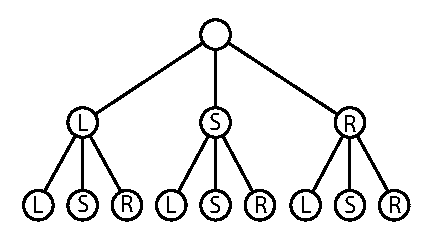
\includegraphics[width=8.5cm]{images/graph_seq_uct.pdf}
\caption{A tree resembling the structure of sequential MCTS. Each node represents a move. The first level represents Player 1 moves and the second level represents Player 2 moves. L,S and R represents the different moves a player can make. L=Left, S=Straight and R=Right.\label{fig:graph_suct}}
\end{center}
\end{figure}

\begin{figure}
\begin{center}
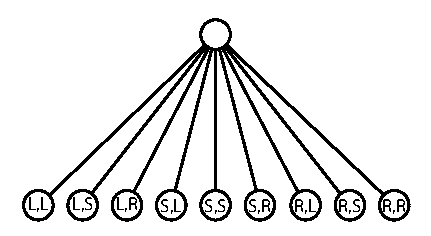
\includegraphics[width=8.5cm]{images/graph_dec_uct.pdf}
\caption{A tree resembling the structure of decoupled MCTS. Each node represents a joint-action consisting of two moves, one for Player 1 and one for Player 2. L,S and R represents the different moves a player can make. L=Left, S=Straight and R=Right. Hence, (L,S) stands for Player1=Left and Player2=Right.\label{fig:graph_duct}}
\end{center}
\end{figure}

\subsection{Decoupled UCB1-Tuned}
\label{subsec:decoupled_ucb1_tuned}
Just as an enhancement can be made by replacing the parameter $C$ by a smart upper bound of the variance of the rewards in UCT~\cite{cig_paper}, it can also be made to DUCT. Each time a node is selected and a joint action is chosen, Equations~\ref{ucb1tuned_ucb} and~\ref{ucb1tuned} are used.

\subsection{EXP3}
\label{subsec:exp3}
To this point, all selection strategies introduced, except DUCT(Mix), are deterministic strategies. DUCT(Mix) and EXP3~\cite{Teytaud11Upper} belong to the group of stochastic selection strategies, which means that there is a random factor involved and that we cannot tell deterministically beforehand which action is going to be chosen. EXP3, as DUCT, always selects joint-actions.\\
EXP3 stores a list of estimated sums of payoffs $\hat{X}_{a^{p}_{k}}$, where $a^{p}_{k}$ mean action $k$, played by player $p$. From the list of payoffs, a policy $P$ is created. The probability of choosing action $a^{p}_{k}$ of policy $P$ is shown in Equation~\ref{exp3_policy}.

\begin{equation}\label{exp3_policy}
P_{a^{p}_{k}}=\frac{e^{\hat{X}_{a^{p}_{k}}}}{\sum\limits_{i \in A_{p}}e^{\hat{X}_{a^{p}_{i}}}},
\end{equation}
where $A_{p}$ is the set of actions from player $p$. Since Equation~\ref{exp3_policy} leads to numerical instability, Equations~\ref{exp3_policy_new} and~\ref{exp3_policy_weight} are used instead. From this policy, a probability $\sigma_{a^{p}_{k}}$ is computed (See Equation~\ref{exp3_distribution}) from which a mixed strategy is played. The final move is chosen in the same way as it was in DUCT(Mix).

\begin{equation}\label{exp3_policy_new}
P^{new}_{a^{p}_{k}}=\frac{e^{\eta\omega(a^{p}_{k})}}{\sum\limits_{i \in A_{p}}e^{\eta\omega(a^{p}_{i})}},
\end{equation}
where $\omega$ can be scaled by some constant $\eta$, but for simplicity $\eta=1$ is chosen. Otherwise $\eta$ can be tuned to increase the performance of EXP3.


\begin{equation}\label{exp3_policy_weight}
\omega(a^{p}_{k})=\hat{X}_{a^{p}_{k}}-argmax_{i \in A_{p}}\hat{X}_{a^{p}_{i}}
\end{equation}

\begin{equation}\label{exp3_distribution}
\sigma_{a^{p}_{k}}=(1-\gamma) \times P^{new}_{a^{p}_{k}} + \frac{\gamma}{|A_{p}|}
\end{equation}

Parameter $\gamma$ can be optimized by tuning it. The update of $\hat{X}_{p}(a_{n})$ after selecting a joint action $(a_{1},a_{2})$, by using the probability $\sigma_{i}(a_{j})$, which returned some simulation result of a play-out $r^{p}_{a_{k_{1}},a_{k_{2}}}$ is shown in Equation~\ref{exp3_update}. The final move is selected by using a mixed strategy by normalizing over the visit counts.

\begin{equation}\label{exp3_update}
\hat{X}_{a^{p}_{k}} = \hat{X}_{a^{p}_{k}} + \frac{r^{p}_{a_{k_{1}},a_{k_{2}}}}{\sigma_{a^{p}_{k}}},
\end{equation}
where $r^{p}_{a_{k_{1}},a_{k_{2}}}$ is the reward of the play-out, when player 1 player chose move $k_{1}$ and player 2 chose move $k_{2}$ and is give in respect to player $p$.

\subsection{Regret Matching}
\label{subsec:rm}
Regret Matching, as EXP3 and DUCT, selects always joint actions. Opposed to the other strategies, Regret Matching stores a matrix $M$ with the estimated mean of the rewards (See Equation~\ref{mat_regret}, where $\bar{X}_{m,n}$ is the sum of the rewards, when selecting the joint action $(a_{1}=m,a_{2}=n)$).

\begin{equation}\label{mat_regret}
M = 
\begin{bmatrix}

\bar{X}_{1,1} && \bar{X}_{2,1} && \bar{X}_{3,1} \\
\bar{X}_{1,2} && \bar{X}_{2,2} && \bar{X}_{3,2} \\
\bar{X}_{1,3} && \bar{X}_{2,3} && \bar{X}_{3,3}

\end{bmatrix}
\end{equation}

Additional to matrix $M$, two lists are stores which keep track of the so called regret of each move from both players ($R_{a^{p}_{k}}$ is the cumulative regret of player $p$ not having taken action $k$). The regret is a value, which indicates how much the player regrets not having played this action. This is the fundamental idea of this selection strategy. With the help of the two lists containing the cumulative regret, a policy ($P_{a^{p}_{k}}$) is created. The policy is created by normalizing over the positive regrets (E.g.: The regrets are: $r_{a^{1}_{1}} = 8.0$, $r_{a^{1}_{2}} = 5.0$ and $r_{a^{1}_{3}} = -4.0$. Then the policies are: $P_{a^{1}_{1}} = \frac{8}{13}$, $P_{a^{1}_{2}} = \frac{5}{13}$ and $P_{a^{1}_{3}} = 0$.)\\
As in EXP3, this policies are used to compute a probability from which a mixed strategy is played (See Equation~\ref{regret_eq}. Variable $\gamma$, as in EXP3, can be tuned to increase performance).

\begin{equation}\label{regret_eq}
\sigma_{a^{p}_{k}}=(1-\gamma) P_{a^{p}_{k}} + \frac{\gamma}{|A_{p}|}
\end{equation}

Initially, all values in matrix $M$ and all values in the regret lists are set to zero. After the play-out is finished and the result ($r^{p}_{a_{m},a_{n}}$) of it gets back propagated, the values in matrix $M$ (See Equation~\ref{update_matrix}) and in the regret lists (See Equation~\ref{update_regret}) have to be updated.

\begin{equation}\label{update_matrix}
%\begin{align}
X_{m,n} = X_{m,n} + r^{p}_{a^{1}_{m},a^{2}_{n}}
%\end{align}
\end{equation}

\begin{equation}\label{update_regret}
%\begin{align}
\forall a^{1}_{i} \in A_{1}, R_{a^{1}_{i}} = R_{a^{1}_{i}} + (\bar{X}_{i,n} - r^{1}_{a_{m},a_{n}})\\
\forall a^{2}_{i} \in A_{2}, R_{a^{2}_{i}} = R_{a^{2}_{i}} + (\bar{X}_{m,i} - r^{2}_{a_{m},a_{n}})
%\end{align}
\end{equation}

The final move is selected as in DUCT(Mix) and EXP3 by using a mixed strategy by normalizing over the visit counts. 

\section{Experiments}
\label{sec:experiments}
In this section the different selection strategies, which were proposed in Section~\ref{sec:selection_strategies} are tested. Because the framework, which was implemented by Teuling~\cite{teuling_tron}, used for this experiments is based on sequential UCT, DUCT, EXP3 and Regret Matching were not optimally implemented. Therefore it would be an unfair comparison, if all agents would have the same thinking time. In order to make it a fair comparison, each agent is allowed to simulate a fixed number of simulations. In the case of this experiment the number is set to 100,000. The experiments are run on four different boards (Three boards with obstacles on it (See Fig.~\ref{fig:ex_boards}) and an empty board (d)), all with dimensions of 16$\times$16. On each board 200 games are played and, even though all the boards are symmetric, the starting positions are switched after half of the games, to assure that none of the agents are benefiting from starting in a certain position. The play-out strategy, which is used in all experiments is the random strategy with play-out cut-off as an enhancement. Also, the expansion strategy uses the predictive expansion strategy.\\
Some parameters are tuned in Subsection~\ref{subsec:parameter_tuning} and the several selection strategies introduced in this paper, are tested against each other in a round-robin tournament in Subsection~\ref{subsec:round_robin}. In addition another round-robin tournament is conducted on a smaller 6$\times$6 board to see how the results differ from the ones conducted in the round-robin tournament on the large boards.

\begin{figure}[t]
\begin{center}
\includegraphics[width=8.5cm]{images/boards.png}
\caption{Four different boards are used for the experiments in the round-robin tournament. a,b and c, as well as the empty board, d, of the same size.\label{fig:ex_boards}}
\end{center}
\end{figure}

\subsection{Parameter Tuning}
\label{subsec:parameter_tuning}
In the beginning, some parameters ($C$ and $T$ in UCT and $\gamma$ in EXP3 and Regret Matching) are tuned. This is done, to assure that the different strategies perform optimally. As reference constants, values are used, which were taken from different sources~\cite{teuling_tron,cig_paper}. Parameter $C$, which is used in UCB1 (See Equation~\ref{uct}) was tuned, by letting a UCT player playing games against a MCTS player with a random selection and a random play-out strategy. After 10 games the value of the parameter $C$ was slightly increased or decreased, depending on how strong the UCT player played. Starting with the reference constant, 120 games were played in order to find a value for $C$ which did not change significantly anymore.\\
The parameter $T$ used in UCT and UCB1-Tuned, which is the threshold before either UCT or UCB1-Tuned is applied as a selection strategy was tuned in the same way as the parameter $C$. This parameter tuning showed the same result as shown by Teuling~\cite{teuling_tron}, namely that the parameter $T$ does not influence the performance of UCT and UCB1-Tuned.\\
The parameter $\gamma$ of EXP3 and Regret Matching was also tuned in the same way as the parameter $C$ with the only difference, that $\gamma$ must be in the interval of $[0,1]$.\\
All the tuned values can be seen in Table~\ref{table:parameter_tuning}.

\begin{table}[b]\footnotesize
\caption{Results of the parameter-tuning of parameters $C$ and $T$ from the UCT Algorithm and from the parameter $\gamma$ of the EXP3 algorithm}
\centering
\begin{tabular}{|c||c|c|}
							\hline
Parameter			& Reference constant		& Tuned value	\\ \hline\hline
$C$				& 10~\cite{teuling_tron}	& 13.2		\\ \hline
$T$				& 30~\cite{teuling_tron}	& 30		\\ \hline
$\gamma$(EXP3)			& 0.36~\cite{cig_paper}		& 0.39		\\ \hline
$\gamma$(Regret Matching)	& 0.36				& 0.31		\\ \hline

\end{tabular}
\label{table:parameter_tuning}
\end{table}

\subsection{Round-Robin Tournament}
\label{subsec:round_robin}
In this subsection, several players using different selection strategies are tested. In Table~\ref{table:round_robin} the results of the games on all four maps are seen and Table~\ref{table:round_robin_total} shows the average performance of all players.

\begin{table*}\scriptsize
\caption{Results of the different selection strategies playing on Board a,b,c and d.}
\centering
\begin{tabular}{|c||c|c|c|c|c|c|c|c|}
									\hline
  Board a 		& UCT 	& UCB1T		& DUCT(Max)	& DUCT(Mix)	& DUCB1T(Max)	& DUCB1T(Mix)	& EXP3	& RM				\\ 	\hline\hline
  UCT 			&  -	& 61\%		& 51\% 		& 54\%		& 53\%		& 67\%		& 65\%	& 62\%				\\ 	\hline
  UCB1T 		& 39\% 	& - 		& 53\%		& 61\%		& 52\%		& 65\%		& 66\%	& 61\%				\\ 	\hline
  DUCT(Max) 		& 49\% 	& 47\%		& -		& 67\%		& 43\%		& 62\%		& 63\%	& 67\%				\\ 	\hline
  DUCT(Mix) 		& 46\% 	& 39\% 		& 33\%		& -		& 37\%		& 48\%		& 53\%	& 51\%				\\ 	\hline
  DUCB1T(Max)	 	& 47\% 	& 48\% 		& 57\%		& 63\%		& -		& 61\%		& 64\%	& 69\%				\\ 	\hline
  DUCB1T(Mix)	 	& 33\% 	& 35\% 		& 38\%		& 52\%		& 39\%		& -		& 54\%	& 51\%				\\ 	\hline
  EXP3 			& 35\% 	& 34\% 		& 37\%		& 47\%		& 36\%		& 46\%		& -	& 51\%				\\ 	\hline
  RM		 	& 38\%	& 39\% 		& 33\%		& 49\%		& 31\%		& 49\%		& 49\%	& -				\\ 	\hline
\end{tabular}

\begin{tabular}{|c||c|c|c|c|c|c|c|c|}
									\hline
  Board b 		& UCT 	& UCB1T		& DUCT(Max)	& DUCT(Mix)	& DUCB1T(Max)	& DUCB1T(Mix)	& EXP3	& RM				\\ 	\hline\hline
  UCT 			&  -	& 47\%		& 49\%		& 57\%		& 51\%		& 61\%		& 61\%	& 59\%				\\ 	\hline
  UCB1T 		& 53\% 	& - 		& 51\%		& 54\%		& 49\%		& 65\%		& 64\%	& 57\%				\\ 	\hline
  DUCT(Max) 		& 51\% 	& 49\% 		& -		& 54\%		& 51\%		& 58\%		& 54\%	& 52\%				\\ 	\hline
  DUCT(Mix) 		& 43\%	& 46\% 		& 46\%		& -		& 41\%		& 52\%		& 49\%	& 46\%				\\ 	\hline
  DUCB1T(Max)	 	& 49\% 	& 51\% 		& 49\%		& 59\%		& -		& 68\%		& 62\%	& 65\%				\\ 	\hline
  DUCB1T(Mix)	 	& 39\% 	& 35\% 		& 42\%		& 48\%		& 32\%		& -		& 57\%	& 52\%				\\ 	\hline
  EXP3 			& 39\% 	& 36\% 		& 46\%		& 51\%		& 38\%		& 43\%		& -	& 57\%				\\ 	\hline
  RM 			& 41\% 	& 43\% 		& 48\%		& 54\%		& 35\%		& 48\%		& 43\%	& -				\\ 	\hline
\end{tabular}

\begin{tabular}{|c||c|c|c|c|c|c|c|c|}
									\hline
  Board c 		& UCT 	& UCB1T		& DUCT(Max)	& DUCT(Mix)	& DUCB1T(Max)	& DUCB1T(Mix)	& EXP3	& RM				\\ 	\hline\hline
  UCT 			&  -	& 37\% 		& 81\%		& 89\%		& 84\%		& 96\%		& 71\%	& 72\%				\\ 	\hline
  UCB1T 		& 63\% 	& - 		& 79\%		& 71\%		& 88\%		& 89\%		& 73\%	& 70\%				\\ 	\hline
  DUCT(Max) 		& 19\% 	& 21\% 		& -		& 58\%		& 41\%		& 52\%		& 69\%	& 61\%				\\ 	\hline
  DUCT(Mix) 		& 11\% 	& 29\% 		& 42\%		& -		& 39\%		& 49\%		& 51\%	& 51\%				\\ 	\hline
  DUCB1T(Max)	 	& 16\% 	& 12\% 		& 59\%		& 61\%		& -		& 59\%		& 68\%	& 64\%				\\ 	\hline
  DUCB1T(Mix)	 	& 4\%  	& 11\% 		& 48\%		& 51\%		& 41\%		& -		& 50\%	& 58\%				\\ 	\hline
  EXP3 			& 29\% 	& 27\% 		& 31\%		& 49\%		& 32\%		& 50\%		& -	& 49\%				\\ 	\hline
  RM 			& 28\% 	& 30\% 		& 39\%		& 49\%		& 36\%		& 42\%		& 51\%	& -				\\ 	\hline
\end{tabular}

\begin{tabular}{|c||c|c|c|c|c|c|c|c|}
									\hline
  Board d 		& UCT 	& UCB1T		& DUCT(Max)	& DUCT(Mix)	& DUCB1T(Max)	& DUCB1T(Mix)	& EXP3	& RM				\\ 	\hline\hline
  UCT 			&  -	& 52\%		& 48\%		& 51\%		& 50\%		& 64\%		& 67\%	& 65\%				\\ 	\hline
  UCB1T 		& 48\% 	& - 		& 45\%		& 57\%		& 53\%		& 67\%		& 59\%	& 67\%				\\ 	\hline
  DUCT(Max) 		& 52\% 	& 55\% 		& -		& 60\%		& 49\%		& 61\%		& 59\%	& 62\%				\\ 	\hline
  DUCT(Mix) 		& 49\% 	& 43\% 		& 40\%		& -		& 41\%		& 55\%		& 50\%	& 49\%				\\ 	\hline
  DUCB1T(Max)	 	& 50\% 	& 47\% 		& 51\%		& 59\%		& -		& 57\%		& 64\%	& 68\%				\\ 	\hline
  DUCB1T(Mix)	 	& 36\% 	& 33\% 		& 39\%		& 45\%		& 43\%		& -		& 51\%	& 49\%				\\ 	\hline
  EXP3 			& 33\% 	& 41\% 		& 41\%		& 50\%		& 36\%		& 49\%		& -	& 52\%				\\ 	\hline
  RM 			& 35\% 	& 23\% 		& 38\%		& 51\%		& 32\%		& 51\%		& 48\%	& -				\\ 	\hline
\end{tabular}
\caption*{UCB1T=UCB1-Tuned, DUCB1T(Max)=DUCB1-Tuned(Max), DUCB1T(Mix)=DUCB1-Tuned(Mix), RM=Regret Matching}
\label{table:round_robin}
\end{table*}

\begin{table*}\scriptsize
\caption{Average results of the different selection strategies playing against each other.}
\centering
\begin{tabular}{|c||c|c|c|c|c|c|c|c|}
									\hline
  Total 		& UCT 	& UCB1T		& DUCT(Max)	& DUCT(Mix)	& DUCB1T(Max)	& DUCB1T(Mix)	& EXP3	& RM				\\ 	\hline\hline
  UCT 			&  -	& 49\%		& 57\%		& 63\%		& 60\%		& 72\%		& 66\%	& 64\%				\\ 	\hline
  UCB1T 		& 51\% 	& - 		& 57\%		& 61\%		& 61\%		& 71\%		& 65\%	& 63\%				\\ 	\hline
  DUCT(Max) 		& 43\% 	& 43\% 		& -		& 60\%		& 46\%		& 58\%		& 61\%	& 60\%				\\ 	\hline
  DUCT(Mix) 		& 37\% 	& 39\% 		& 40\%		& -		& 40\%		& 51\%		& 51\%	& 49\%				\\ 	\hline
  DUCB1T(Max)	 	& 40\% 	& 39\% 		& 54\%		& 60\%		& -		& 61\%		& 65\%	& 67\%				\\ 	\hline
  DUCB1T(Mix)	 	& 18\% 	& 19\% 		& 42\%		& 49\%		& 39\%		& -		& 53\%	& 52\%				\\ 	\hline
  EXP3 			& 34\%	& 35\% 		& 39\%		& 49\%		& 35\%		& 47\%		& -	& 52\%				\\ 	\hline
  RM		 	& 36\% 	& 37\%		& 40\%		& 51\%		& 33\%		& 48\%		& 48\%	& -				\\ 	\hline
\end{tabular}
\caption*{UCB1T=UCB1-Tuned, DUCB1T(Max)=DUCB1-Tuned(Max), DUCB1T(Mix)=DUCB1-Tuned(Mix), RM=Regret Matching}
\label{table:round_robin_total}
\end{table*}

From Table~\ref{table:round_robin_results} we can see, that the sequential UCT and UCB1-Tuned selection strategies perform best. The Max versions of the decoupled UCT and UCB1-Tuned strategy still performs reasonably well ($>50\%$). All the other strategies, which include the Mix versions of the decoupled UCT and UCB1-Tuned, as well as EXP3 and Regret Matching, perform not that well ($<50\%$).\\
Furthermore it stands out that on Board c, the sequential MCTS out performs  the decoupled versions of MCTS.

The same selection strategies were tested again against each other in another round-robin tournament, which will be played on a 6$\times$6 board. From the results in Table~\ref{table:rr_small} can be seen, that deterministic selection strategies are still doing better that stochastic ones. But, stochastic strategies perform better on the 6$\times$6 board than on the larger 16$\times$16 board.

\subsection{Discussion}
\label{subsec:discussion}

The experiments revealed that the parameter $C$ of the UCT selection strategy was optimal at 13.2. Usually, the parameter $C$ is fairly low, but in Tron, there are only 3 possible moves, therefore it is beneficial to know where all three moves would lead us. A high $C$ parameter ensures that the exploration of all nodes is given, which explains the result of the high $C$ parameter.\\
The parameter $T$ of the UCT and UCB1-Tuned selection strategy was tuned. After some experiments, the tuning was stopped, because it did not seem to have much impact on the result of the selection strategies. Therefore, 30 is still used for the parameter $T$. The parameter $\gamma$ from the EXP3 and Regret Matching selection strategy was tuned to 0.39 and 0.31, respectively, to increase performance of those strategies.\\
The round-robin tournament, in which every selection strategy played against each other, showed that the sequential UCB1-Tuned algorithm wins on average 63\% of its games and is therefore the winner of the tournament. Further it may be concluded, that the sequential strategies perform better than the decoupled strategies, which is especially visible on Board c (See Table~\ref{table:round_robin}), where the UCT and UCB1-Tuned only lost 4\%-19\% of its games against all DUCT strategies and only 28\%-29\% against EXP3 and Regret Matching, respectively. Additionally, it can be concluded that deterministic selection strategies perform superior than stochastic selection strategies on 16$\times$16 boards (All deterministic strategies win $>50\%$ and all stochastic win $<50\%$ of their matches). Already the selection strategies, which are deterministic, but only use a stochastic process to determine their final move, such as DUCT(Mix) and DUCB1-Tuned(Mix), perform way weaker than their counterparts DUCT(Max) and DUCB1-Tuned(Max).\\
Furthermore, the round-robin tournament on the smaller 6$\times$6 board showed, that if a smaller board is used, the performance of the deterministic strategies decrease and the performance of the stochastic strategies increase. This indicates, that as soon as both players come closer together, using a stochastic strategy might be more suitable than a deterministic one. This phenomenon is illustrated in Figure~\ref{fig:stochastic}, where both players have two possible moves. If both players choose $a^{p}_{1}$ (``Left''), Player 1 wins and if both players choose $a^{p}_{2}$ (``Right''), Player 1 also wins. Therefore it might be beneficial for Player 2 to play with a mixed strategy, where the probabilities for choosing actionfor $a^{2}_{1}=0.5$ and for $a^{2}_{2}=0.5$.

\begin{figure}
\begin{center}
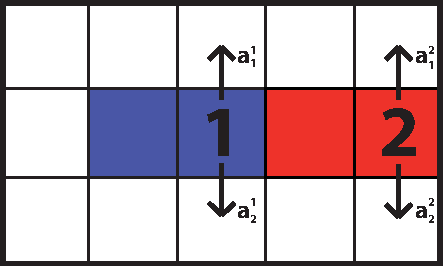
\includegraphics[width=8.5cm]{images/stochastic.pdf}
\caption{A Position, which indicates that mixing strategies is important.}
\label{fig:stochastic}
\end{center}
\end{figure}

\section{Conclusion and Future Research}
\label{sec:conclusion}

\begin{table}[h]\scriptsize
\caption{Results of the different selection strategies playing against each other. a,b,c and d stand for the four different boards, which are used in the round-robin tournament. $\pm$ refers to 95\% confidence intervals.}
\centering
\begin{tabular}{|c||c|c|c|c|c|}
									\hline
	Selection Strategy	& a 		  & b 		  & c 		  & d 		  & Total 	\\ \hline
	UCB1-Tuned		      & 57\%	  & 58\%		& 78\%		& 58\%		& 63$\pm$1.26\%		\\ \hline
	UCT			            & 59\%		& 55\%		& 76\%		& 57\%		& 61$\pm$1.28\%		\\ \hline
	DUCB1-Tuned(Max)	  & 58\%		& 58\%		& 48\%		& 57\%		& 55$\pm$1.30\%		\\ \hline
	DUCT(Max)		        & 56\%		& 53\%		& 37\%		& 57\%		& 51$\pm$1.31\%		\\ \hline
	DUCT(Mix)		        & 44\%		& 46\%		& 39\%		& 47\%		& 45$\pm$1.30\%		\\ \hline
	DUCB1-Tuned(Mix)	  & 43\%		& 44\%		& 38\%		& 42\%		& 42$\pm$1.29\%		\\ \hline
	EXP3			          & 41\%		& 44\%		& 38\%		& 43\%		& 42$\pm$1.29\%		\\ \hline
	Regret Matching		  & 41\%		& 44\%		& 39\%		& 40\%		& 41$\pm$1.28\%		\\ \hline
\end{tabular}
\label{table:round_robin_results}
\end{table}

\begin{table*}\scriptsize
\caption{Results of the different selection strategies playing against each other on a 6$\times$6 board. $\pm$ refers to 95\% confidence intervals.}
\centering
\begin{tabular}{|c||c|c|c|c|c|c|c|c|c|}
									\hline
	6$\times$6 Board	& UCB1T 	& UCT		& DUCT(Max)	& DUCB1T(Max)	& DUCT(Mix)	& DUCB1T(Mix)	& RM	& EXP3	& Total			\\ \hline
	UCB1T							& -				& 52\%	& 59\%			& 62\%				& 59\%			& 62\%				& 57\%& 61\%	& 59$\pm$2.57\%		\\ \hline
	UCT								& 48\%		& -			& 55\%			& 61\%				& 57\%			& 56\%				& 60\%& 59\%	& 57$\pm$2.56\%		\\ \hline
	DUCT(Max)					& 41\%		& 45\%	& -					& 48\%				& 56\%			& 56\%				& 54\%& 60\%	& 52$\pm$2.62\%		\\ \hline
	DUCB1T(Max)				& 38\%		& 39\%	& 52\%			& -						& 56\%			& 57\%				& 63\%& 61\%	& 52$\pm$2.62\%		\\ \hline
	DUCT(Mix)					& 41\%		& 43\%	& 44\%			& 44\%				& -					& 53\%				& 50\%& 49\%	& 47$\pm$2.61\%		\\ \hline
	DUCB1T(Mix)				& 38\%		& 44\%	& 44\%			& 43\%				& 43\%			& -						& 51\%& 54\%	& 46$\pm$2.61\%		\\ \hline
	RM								& 43\%		& 40\%	& 46\%			& 37\%				& 50\%			& 46\%				& -		& 46\%	& 46$\pm$2.61\%		\\ \hline
	EXP3							& 39\%		& 41\%	& 40\%			& 39\%				& 51\%			& 41\%				& 54\%& -			& 44$\pm$2.60\%		\\ \hline
\end{tabular}
\caption*{UCB1T=UCB1-Tuned, DUCB1T(Max)=DUCB1-Tuned(Max), DUCB1T(Mix)=DUCB1-Tuned(Mix), RM=Regret Matching}
\label{table:rr_small}
\end{table*}

In this paper, several selection strategies for the selection phase were introduced, including the deterministic strategies UCT, UCB1-Tuned, DUCT(Max) and DUCB1-Tuned(Max) and the stochastic strategies DUCT(Mix), DUCB1-Tuned(Mix), EXP3 and Regret Matching. All these enhancements were tested in the game of Tron on different boards to see which strategies perform better than others.\\
Overall, the round-robin tournament showed, that UCB1-Tuned performs the best in the game of Tron. Furthermore the experiments showed, that deterministic strategies are superior to stochastic ones, but also that the performance of stochastic strategies increases as the board gets smaller. It also showed, that the layout of the board has great influences on the outcome of a game.\\
For future research, more experiments with different boards are required, in order to determine why some boards (as Board c) create more difficulties for the decoupled strategies.\\
In addition, the selection strategy EXP3 can be enhanced by tuning parameter $\eta$, which was set to $\eta=1$ for simplicity.\\
Moreover, a hybrid selection strategy should be tested, which uses a deterministic strategy if both players are far away from each other and a stochastic one as soon as both players come fairly close to each other. This hybrid selection strategy would indicate, if the assumption made in this paper, that stochastic strategies perform better when both players are close to each other, is correct.



\bibliographystyle{plain}
\bibliography{sm-tron}



\end{document}








